\def\baselinestretch{1}
 \chapter{Financial Engineering}


\section{Modeling High Dimensional Financial Instruments in Real
Time. How to build a TV for RUT \& SPX} In statistical
thermodynamics, infinite systems exhibit scaling behavior that
may break down in a finite setting.  A power law correlation at
a critical point is limited in a finite system while the
mathematics of the infinite system give a singularity at the
critical point.  The long range dependence in real systems
breaks down across regime change.  Essentially, investors
forget. Annealing and hysteresis models from solid state
physics could be employed to explain bubble behavior and market
memory.  Of particular interest are models of random systems
exhibiting long range interactions, critical phenomena, and
frustration. Frustration is an important concept in social
systems. Many competing interests with differing utility
functions making decisions under uncertainty in a complex
environment can lead to bubbles, crashes, and hysteresis. An
example, consider a basket of equities $B =\{S_i\}$ weighted by
$\omega=\{\omega_i\}$. Suppose options are traded on $B$ and
its components, and that we have a set of exogenous driving
factors for the price evolution of the basket $\{\eta_j\}$.

The images below were obtained by fitting high frequency
historical pricing data to a generalized multivariate
elliptical model for returns.  Models were fit for daily, five
minute, and tic interval.

\begin{tabular}[IWM Correlation Matrix and corresponding eigenvalue
distribution.]{ |c|c| }
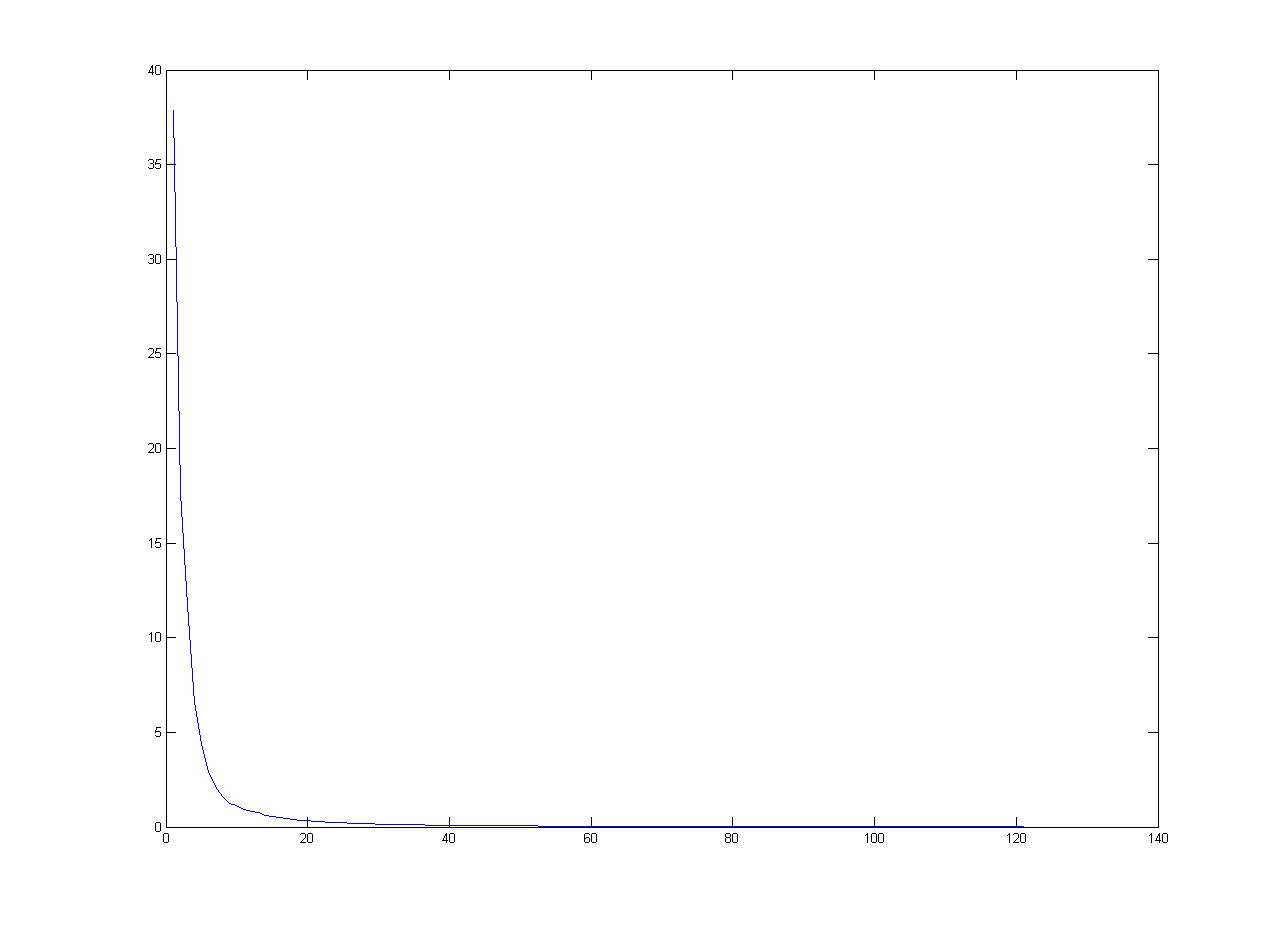
\includegraphics[width=3in,height=3in]{images/RealTimeFinancialTSMining/iwm_day_pca_eigen_var_desc.jpg} &
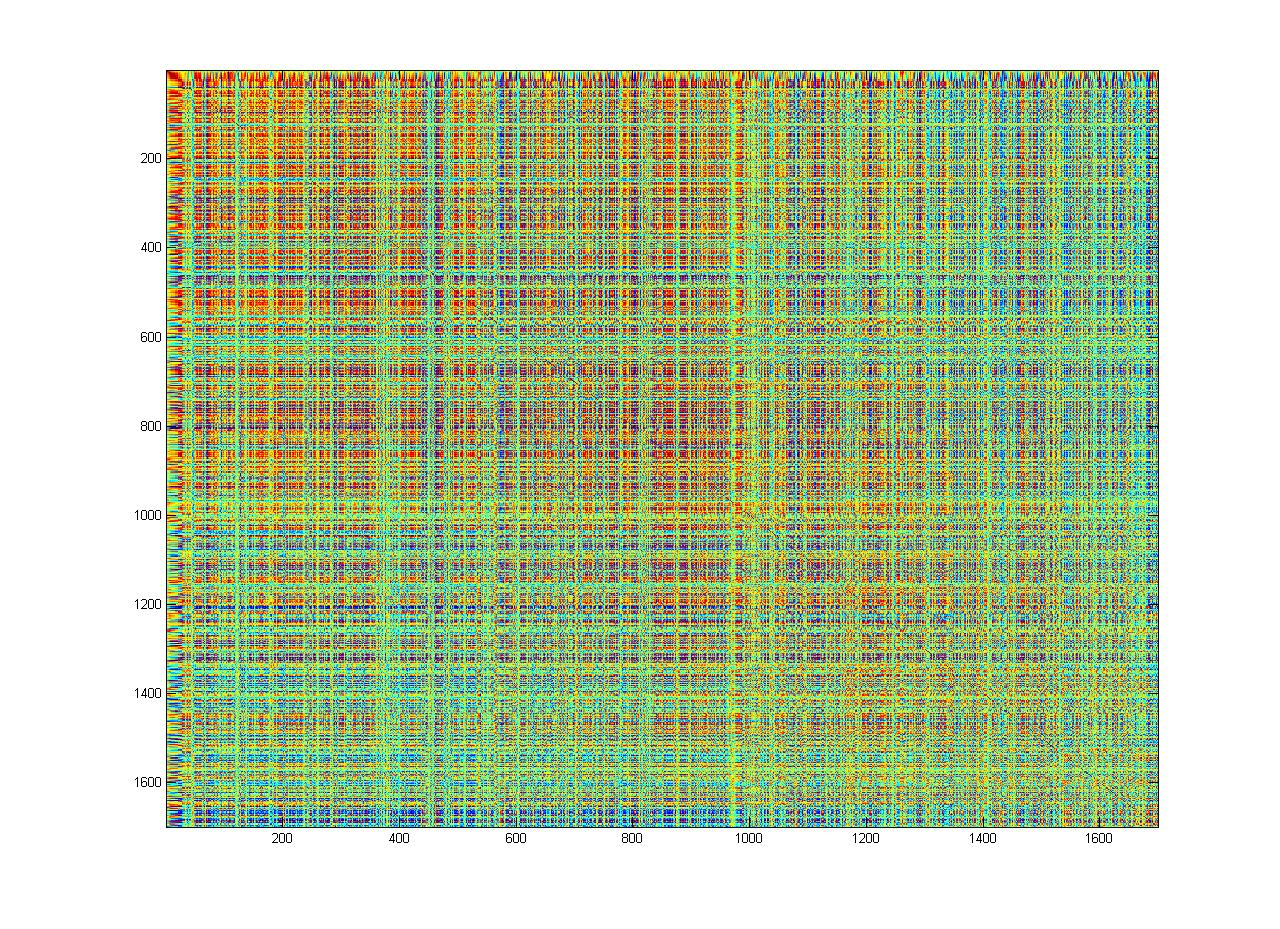
\includegraphics[width=3in,height=3in]{images/RealTimeFinancialTSMining/iwm_day_price_corr.jpg}
\end{tabular}


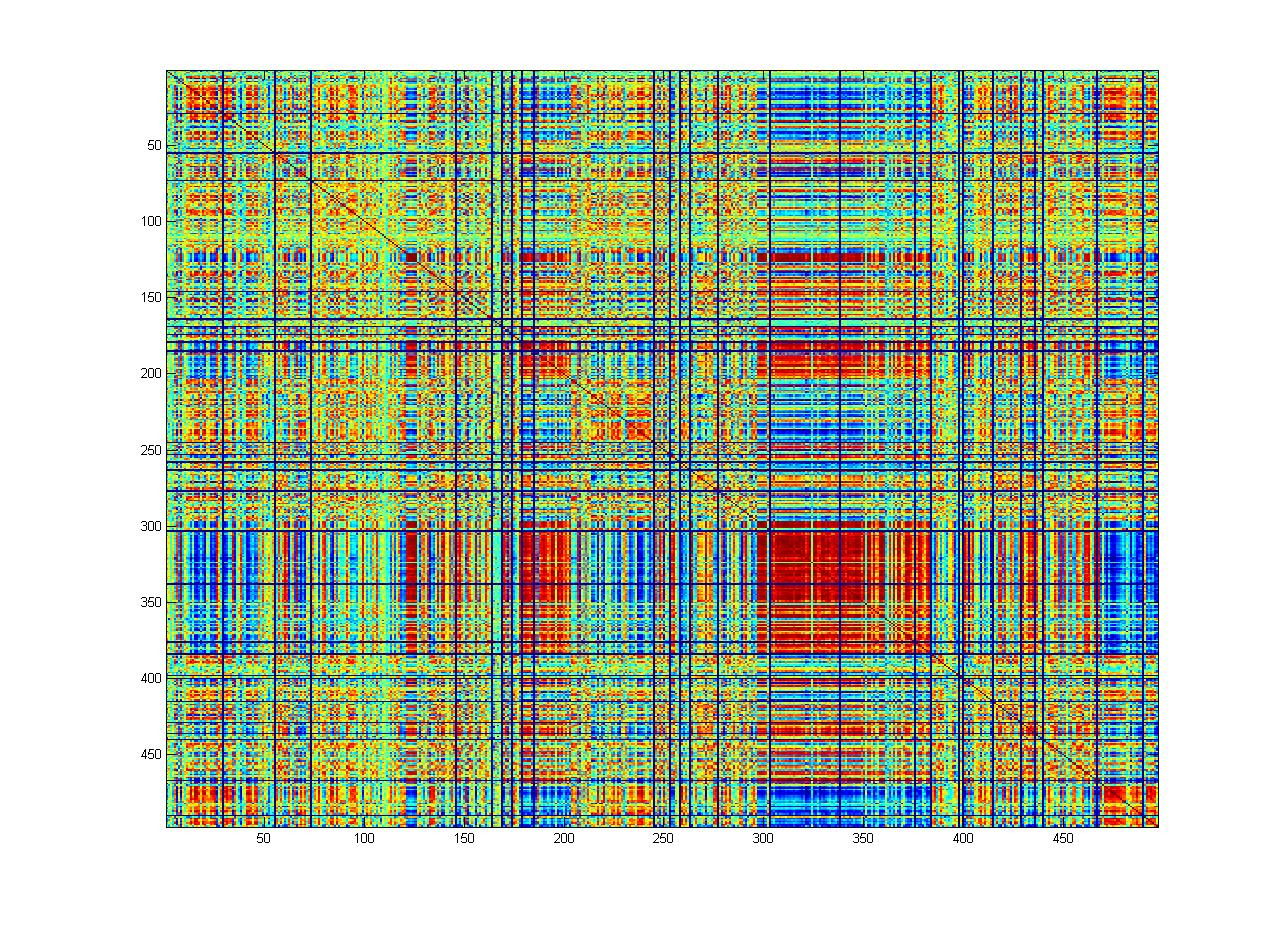
\includegraphics[width=3in,height=3in]{images/RealTimeFinancialTSMining/spy_day_price_corr.jpg}
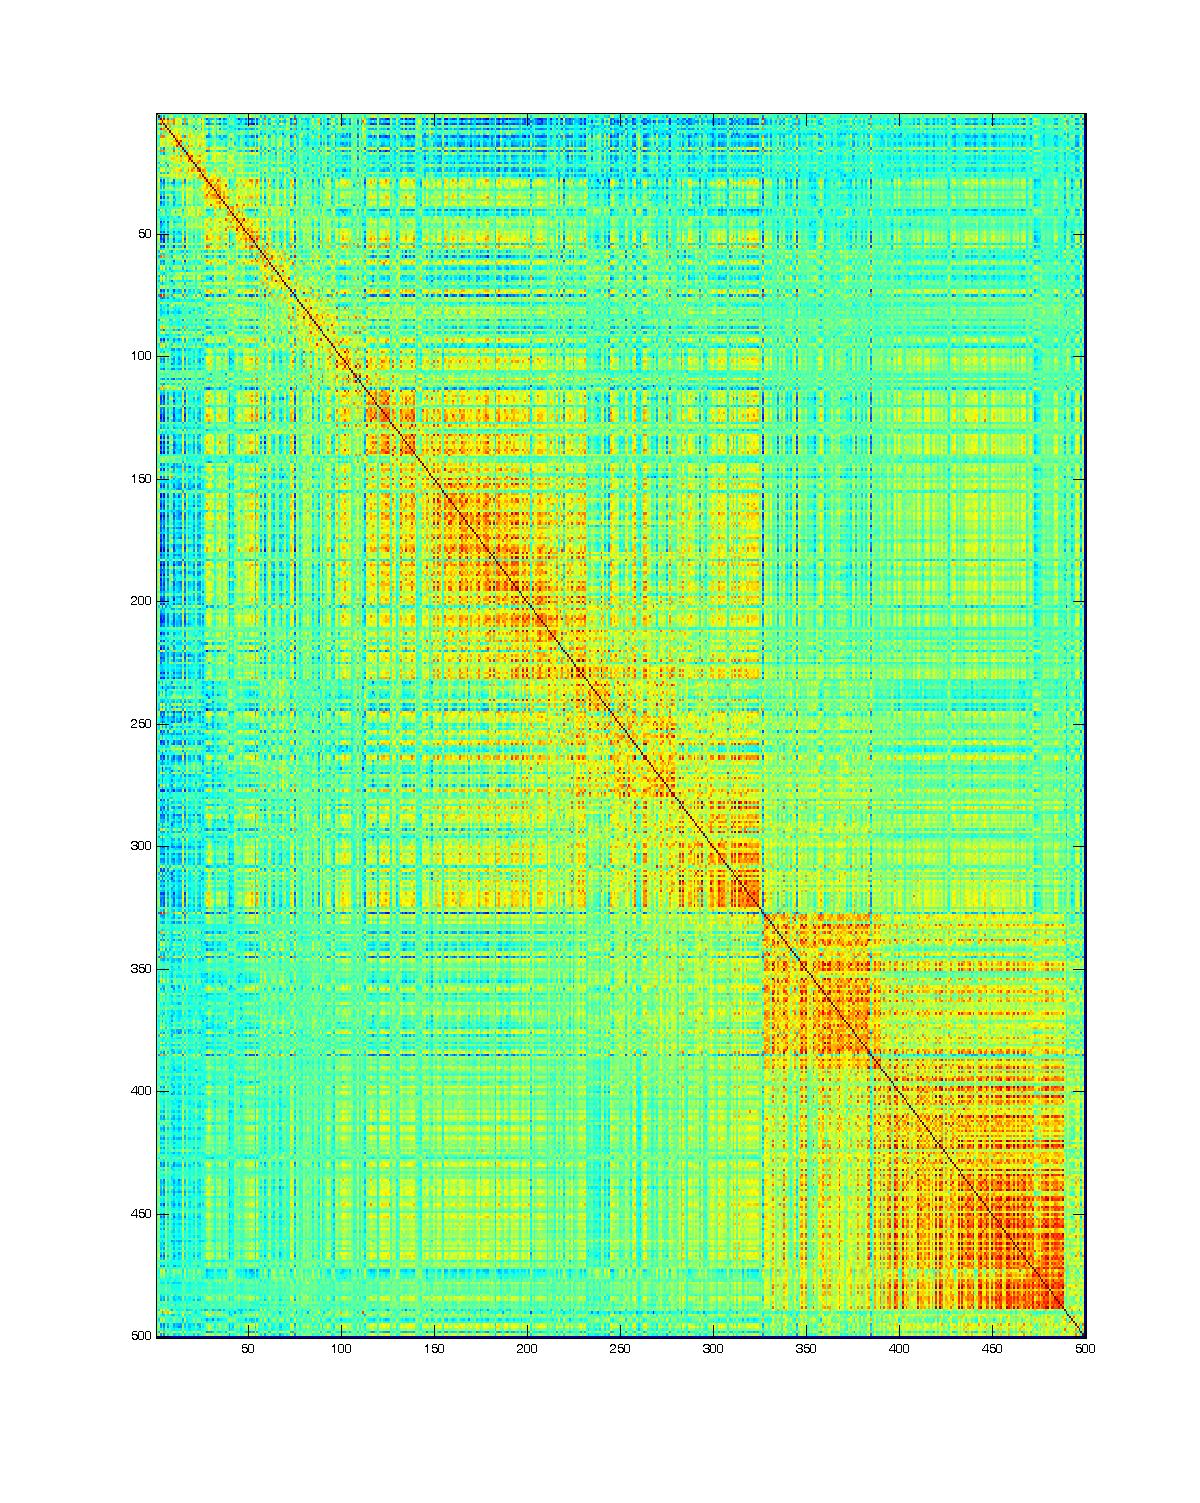
\includegraphics[width=3in,height=3in]{images/RealTimeFinancialTSMining/spy_wk_price_corr.jpg}

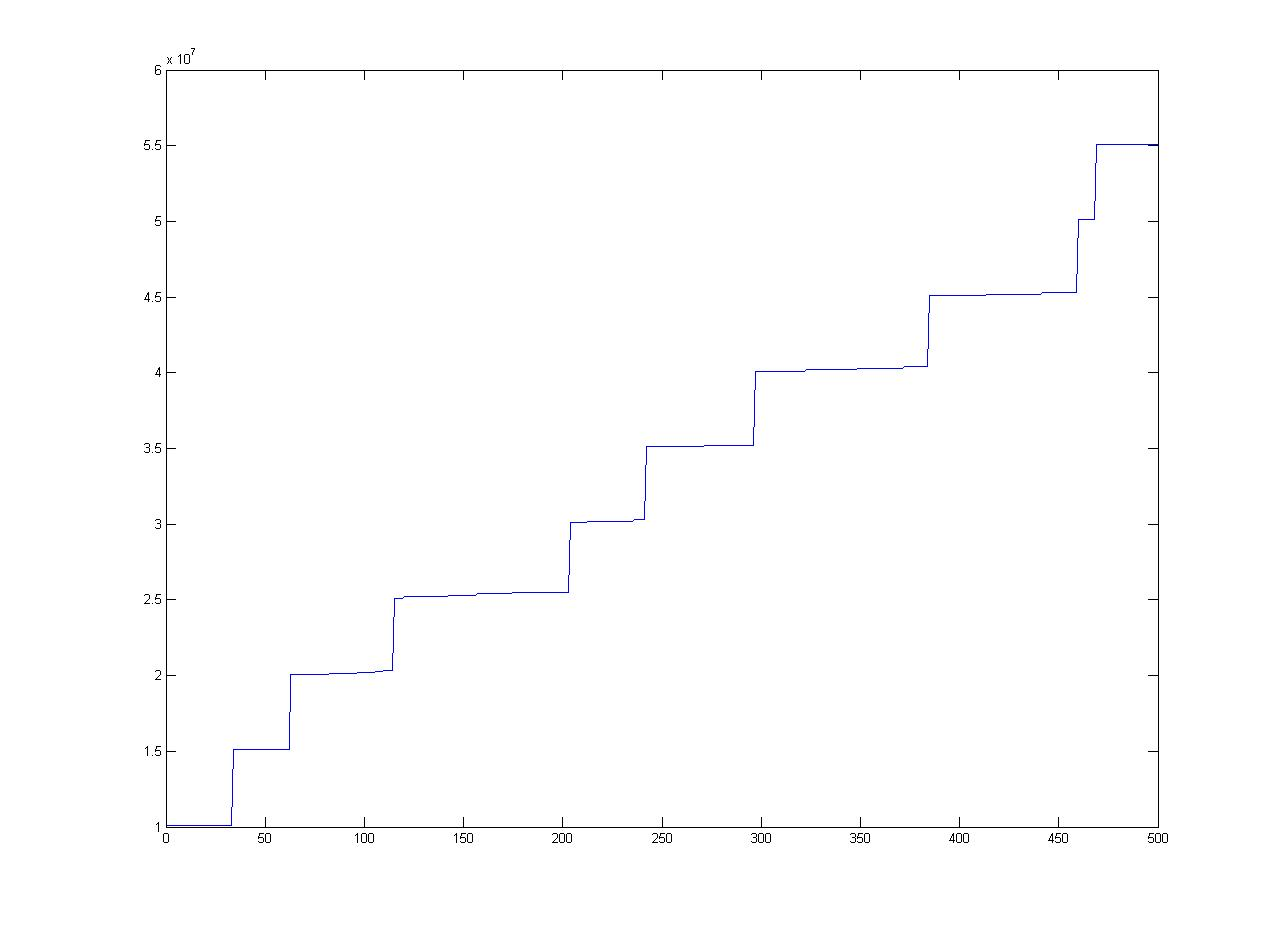
\includegraphics[width=3in,height=3in]{images/RealTimeFinancialTSMining/spy_industrycodes_corr.jpg}

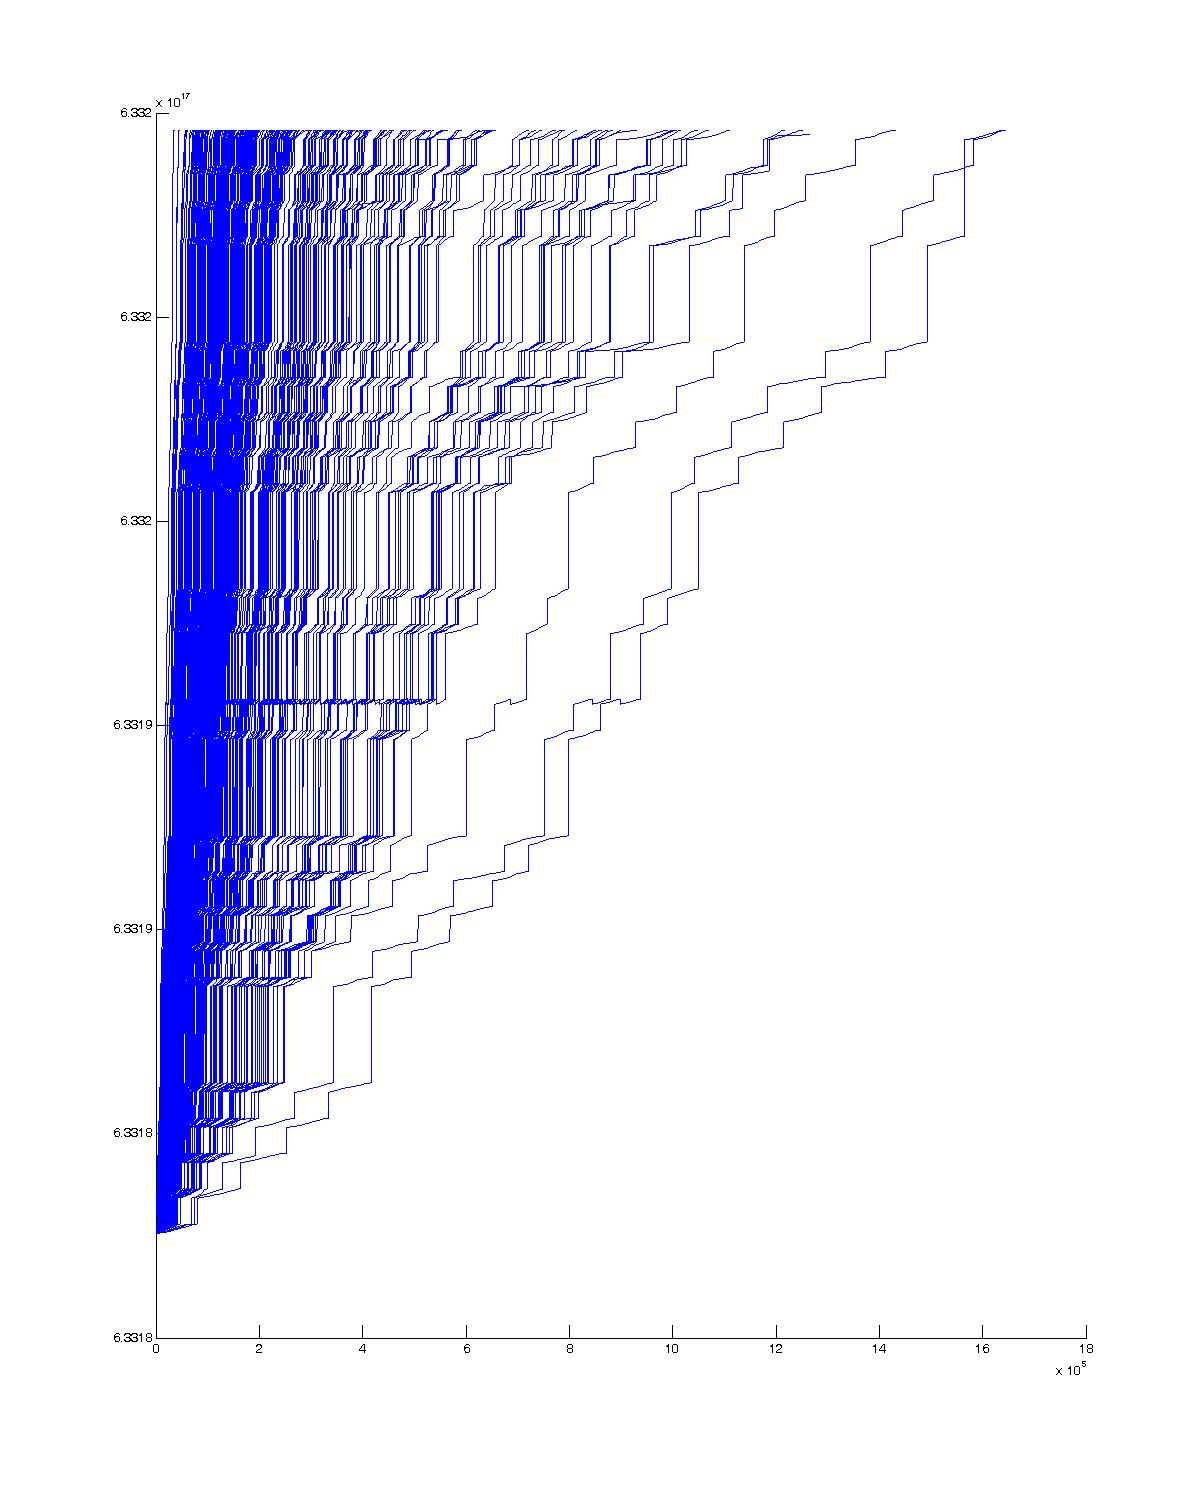
\includegraphics[width=3in,height=3in]{images/RealTimeFinancialTSMining/tics072007_time.jpg}





\section{Time Series Analysis}
$X_{t}$ is a stochastic random process.  If $E [X_{t} ] = \mu$
and $COV[ X_{t}, X_{t+k}] = \gamma_{k}$ are independent of $t$,
then the process is second order stationary.  Define The
autoccorrelation function (ACF) $\rho_{k}=
\frac{\gamma_{k}}{\gamma_{0}}$.  The fourier transform of the
autocovariance ${\gamma_{k} }$ gives the distribution of
variance over the frequency range $[0, \omega_{Nyquist}]$



\section{Long Range Dependence, Rescaled Range,  and the Hurst
Exponent} Three important methods exist to model the long range
dependence in $X(t)$; autocorrelation analysis, state space
methods relying on embedding fractional differences (bbcsvc
verify), and scaling laws.  To form the rescaled range
statistic, for a series of partial sums of scaled variances.
$\widehat{\mu}(N,t_o) = \frac{1}{N} \sum
\limits_{t=t_o+1}^{t=t_o+N} X(t) \widehat{\sigma}^{2}(N,t_o)=
\frac{1}{N} \sum\limits_{t=t_o+1}^{t=t_o+N} ( X(t) -
\widehat{\mu}(N,t_o))^{2} $ now define the range for the scale
$\tau$ by forming the partial sums of the deviations from the
mean at time $t_o$ resolution at scale $N$
% (bbcrevisit replace notation for N, N is not a good scale variable,
%use something consistent with wavelet notation.
$Y(N,t_o,\tau)=\sum \limits_{t=t_o+1}^{t=t_o+\tau}
X(t)-\widehat{\mu}(N,t_o) \fall t \in [1,N]$ Compute the range
from $max_{\tau}Y(N,t_o,\tau)-min_{\tau} Y(N,t_o,\tau)$ The
$RS$ statistic at $t$ is obtained by rescaling the range of the
process at a scale $N$ by the variance  at that scale and time;
\begin{equation}\label{0.1}  RS(N) =  \frac{\sum
\limits_{t=t_o+1}^{t=t_o+N}R(N,t_o)}{\sum
\limits_{t=t_o+1}^{t=t_o+N} \widehat{\sigma^{2}}(N,t_o)}
\end{equation}. Assuming a scaling law exists, $RS(N)\approx
(aN)^{H}$  This is the same type of law defined for phase
transitions in solid state statistical physics.  Refer to the
sections on simulated annealing.  When $H=\frac{1}{2}$ we have
standard Brownian motion, $H \in [0, \frac{1}{2})$ implies a
mean reverting process, and $ H \in (\frac{1}{2},1]$ means a
long range dependence exists in the data.

Long Range Dependence (LRD) can be defined for non-Gaussian
stable processes $X(t)= Y(t) + \varepsilon_t$ where
$\varepsilon$ is the noise.  The process $X(t)$ is LRD if
$\rho_{t,s})=Corr(\varepsilon_t, \varepsilon_s) \sim |t-s|^{-H}
(t-s) \rightarrow \infty$.  Alternatively LRD can be defined if
the characteristic function $ \cal{F}(\varepsilon)(\omega) =
\int \limits_{- \infty}^{\infty} p(x) e^{-2 \pi \omega x} dx$
has a pole at zero in $\field(C)$  The characteristic function
plays an important role in proving limit theorems and deriving
estimators for LRD processes.

The approach outlined above has  similarities with methods of
solid state physics. In physics at the critical point for an
infinite system, there exists discontinuities in the
correlation function | long range correlations ] and to get
convergence in the calculations (bbcrevisit which) ] a
renormalizing transform is applied to bbcrevisit.

If $Y_i, \hdots , Y_n$ iid $N(\mu,\sigma)$ and $R= max_i Y_i -
min_i Y_i$, $S^2=\widehat{\sigma}^2$.  $S_i, Y_i$ are
independent and we can forma new random variable called the
Studentized Range, $Q_{n,\nu}=\frac{R}{S}$  It can be used in a
multiple comparison settings.  When $H=frac{1}{2}$ above,

A probability space $ (\Omega, F, P)$


Refs: Dacorgna, Muller GARCH, HARCH IEMA

For FBM we have no Ito calculus.  Care has to be taken when
defining stochastic integrals. Many approaches exist, and no
consensus yet exists on how to properly define such integral.
The difficulties arise in the range $H \in [0, \frac{1}{2})$
where the sample path properties are more irregular than
standard Brownian motion.  By care, we mean deep results form
measure theory and analysis need to be applied.  Ref Embrechts
Selfsimilar Processes.
%(bbcsvc revisit define mean reverting above ),


\section{Copula's }
A copula is a multivariate cumulative distribution function on
$[0, 1]^n$ such that the marginals are uniform on $[0, 1]$.
Sklar's theorem provides

%
%. For any bivariate distribution function H(x, y), let F(x) = H(x,
%8) and G(y) = H(8, y) be the univariate marginal probability
%distribution functions. Then there exists a copula C such that
%(where we have identified the distribution C with its cumulative
%distribution function). The copula contains all of the information
%on the nature of the dependence between the two random variables
%that can be given without the marginal distributions, but gives no
%information on the marginal distributions. In effect the
%information on the marginals and the information on the dependence
%are neatly separated from each other %%

%Of course everyone would expect these formulas to yield corrmax =
%1 and corrmin = .1. The news is that this is not true in general.
%Of course, that is what we are used to expect in  a world of
%normal returns. The result would also hold in the more general
%case of elliptic distributions, but not for other arbitrary
%choices. Looking at the problem from a different viewpoint,
%correlation is an effective way to represent comovements between
%variables if they are linked by linear relationships, but it may
%be severely flawed in the presence of nonlinear links. Readers may
%check this in the simple case of a variable z normally distributed
%and z2 which is obviously perfectly correlated with the first one,
%but has a chi-squared distribution. So, using linear correlation
%to measure the comovements of markets in the presence of
%non-linear relationships may be misleading because it may not
%cover the whole range from .1 to +1 even though two markets are
%moved by the same factor, and so are perfectly dependent. The
%alternative offered by statistics to this shortcoming is the use
%of non-parametric dependence measures, such as Spearman�s $\rho$
%and Kendall�s $\tau$ . The non-parametric feature of these
%measures means that they do not depend on the marginal probability
%distributions. It does not come as a surprise, then, that these
%measures are directly linked to the copula function. In
%particular, it may be proved that the following relationships hold
%
%Sklar's Theorem Let  be a two-dimensional distribution function
%with marginal distribution functions  and . Then there exists a
%copula  such that  Conversely, for any univariate distribution
%functions  and  and any copula , the function  is a
%two-dimensional distribution function with marginals  and .
%Furthermore, if  and  are continuous, then  is unique. %%%%%%%%%%%
%

\section{ Risk}
Risk is classified generally as credit, market, liquidity, and
operational.  Credit risk measures the potential loss due to
the inability of a counterparty to meet obligations.  Credit
risk is classified as that due to credit exposure, the
provability of counterparty default, and the losses given
counterparty default. Liquidity risk is caused by an unexpected
large and stressful negative cash flow over a short period.
Liquidity risk is assumed by individual firms and market
participants.  Firm or market participant in possession of
illiquid assets may have to sell at a discount to meet cash
flow of margin requirements.  Market risk relates to the
uncertainty of future earnings due to market conditions.

VaR is not coherent unless the underlying price process is
normal.  The expected shortfall ES is a more robust risk
measure since it takes into account the information in the tail
of the price process.  VaR calculation requires marking to
market, estimation of the distribution of return process, and
finding a risk measure to calculate the actual risk.  VaR in
practice is typically calculated explicitly via assumptions
such as that specified in the Basil accord, via Monte Carlo
Simulation of future returns, or with historical market data.
The models of \cite{Heston (1993)} and \cite{Merton (1976} are
combined to form the affine jump diffusion framework of Duffie,
Pan, and Singleton (2000).

\subsection{Iterated Exponential Filtering of high frequency TS data}
\begin{tabular}{ |c|c|c|c| }
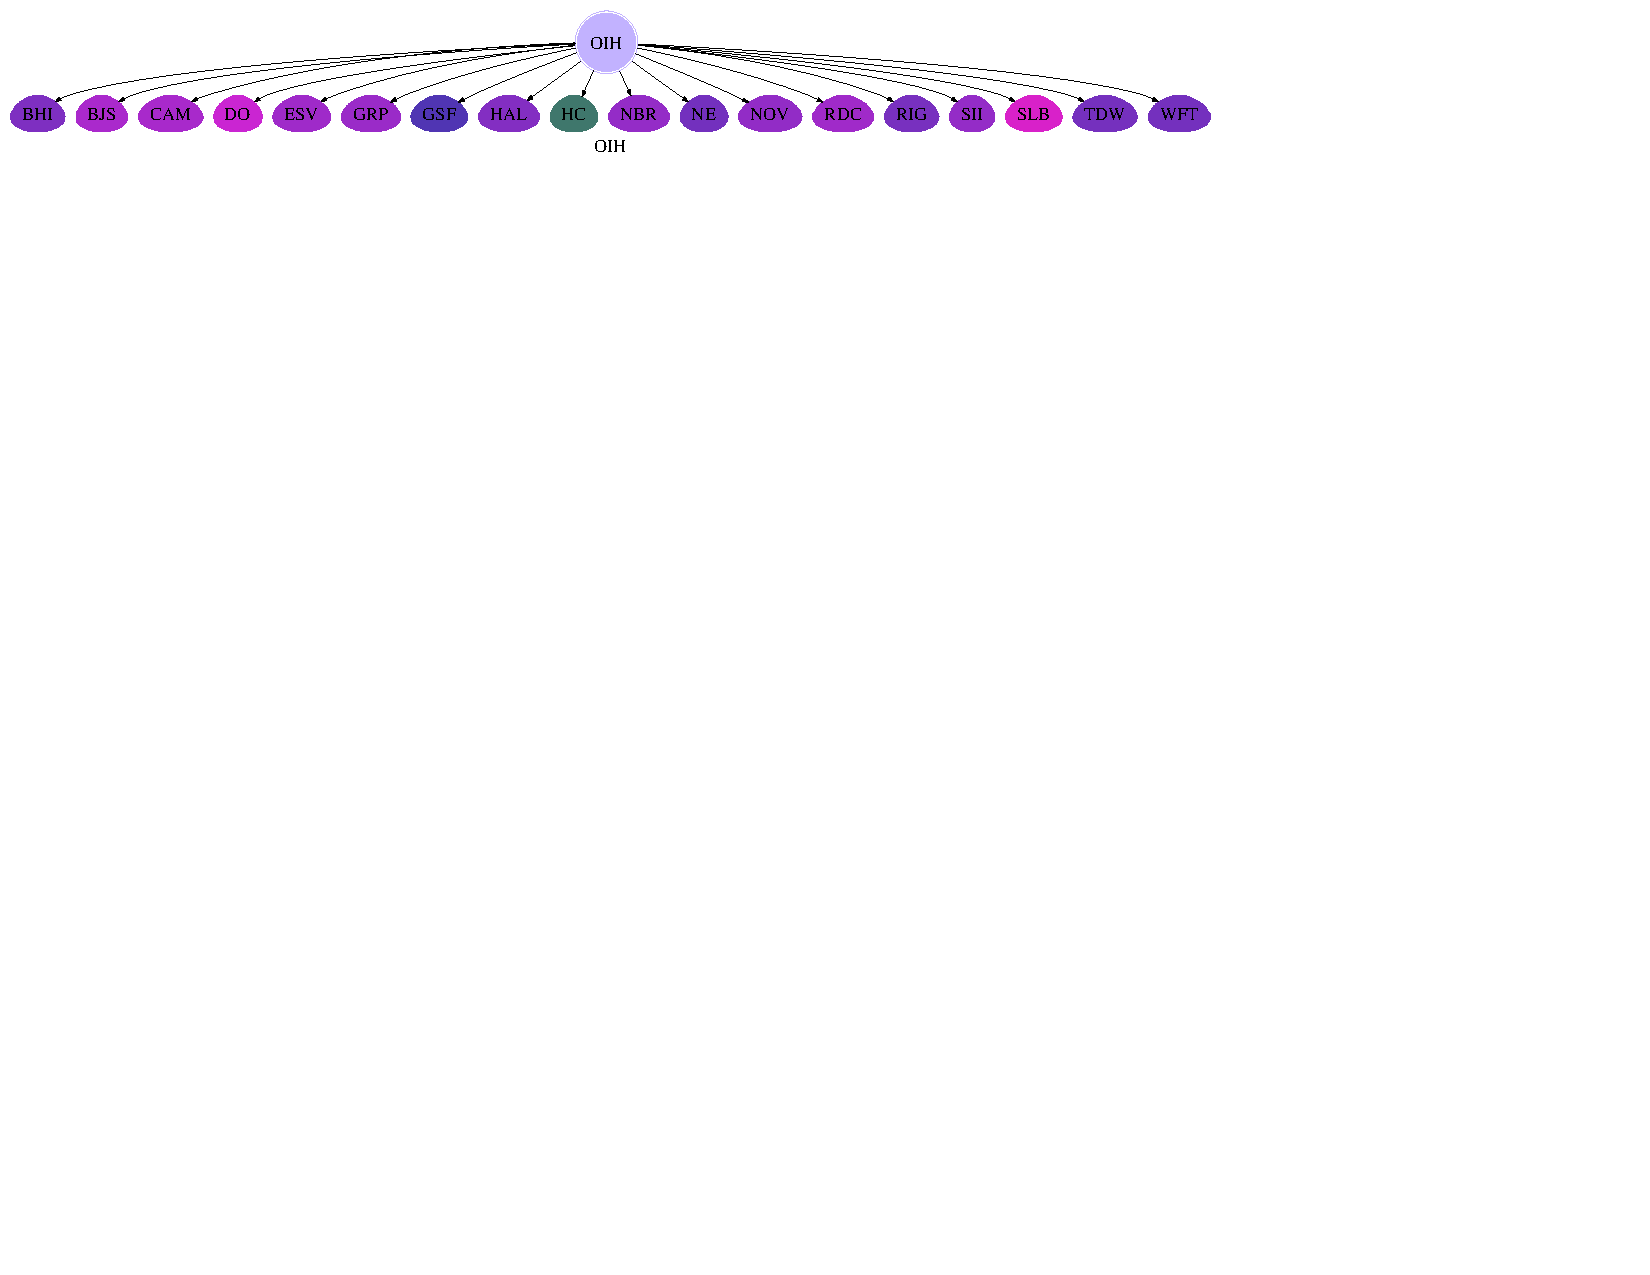
\includegraphics[width=4.0cm,height=4.0cm]{images/RealTimeFinancialTSMining/klTimeSeries/OIHB.pdf}  &
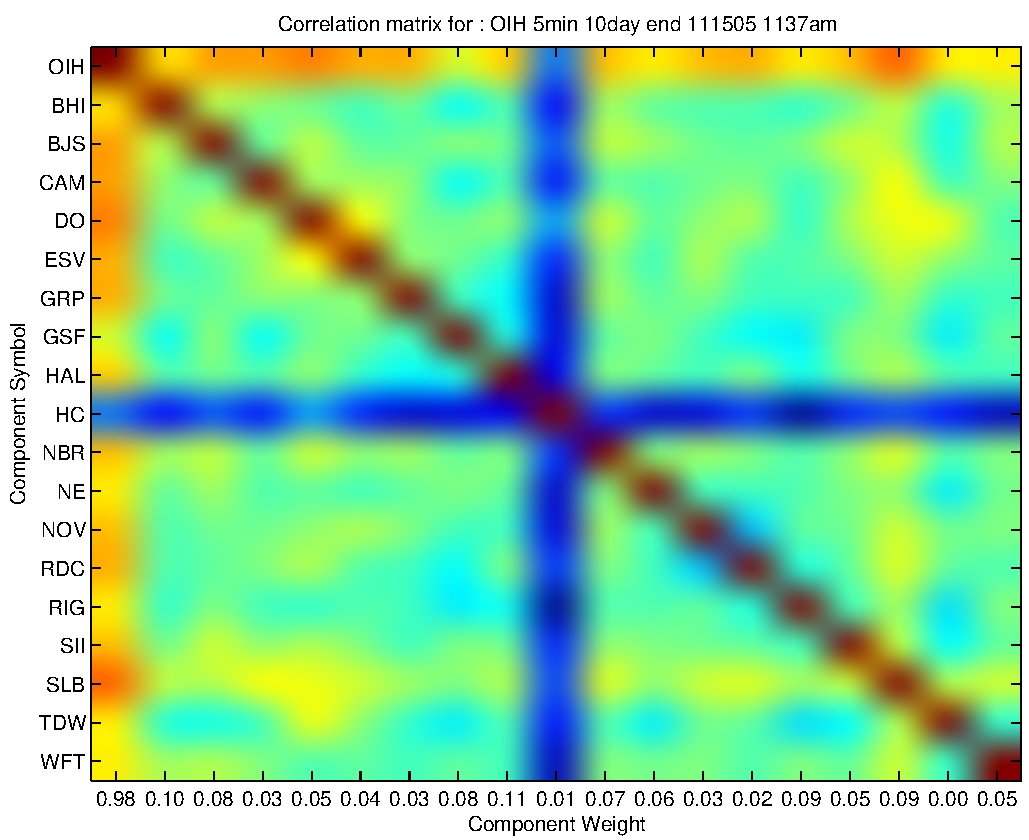
\includegraphics[width=4.0cm,height=4.0cm]{images/RealTimeFinancialTSMining/klTimeSeries/OIHBCorr.pdf} &
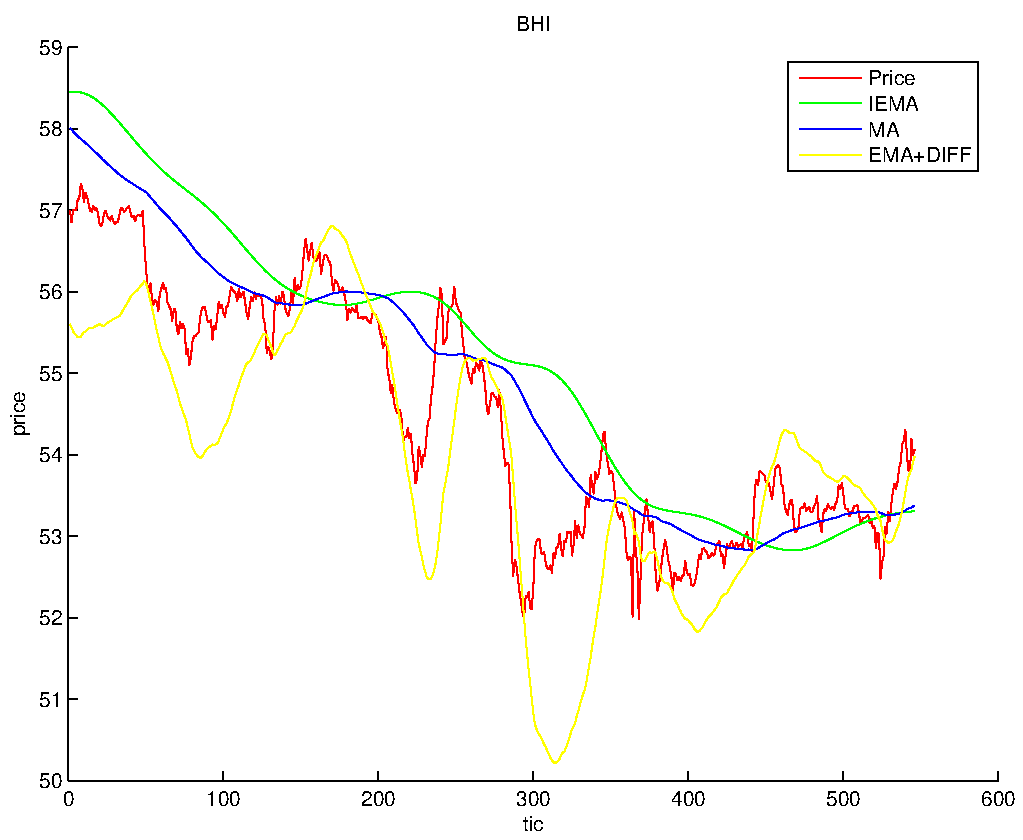
\includegraphics[width=4.0cm,height=4.0cm]{images/RealTimeFinancialTSMining/klTimeSeries/BHIFilteredPriceSeries.pdf} &
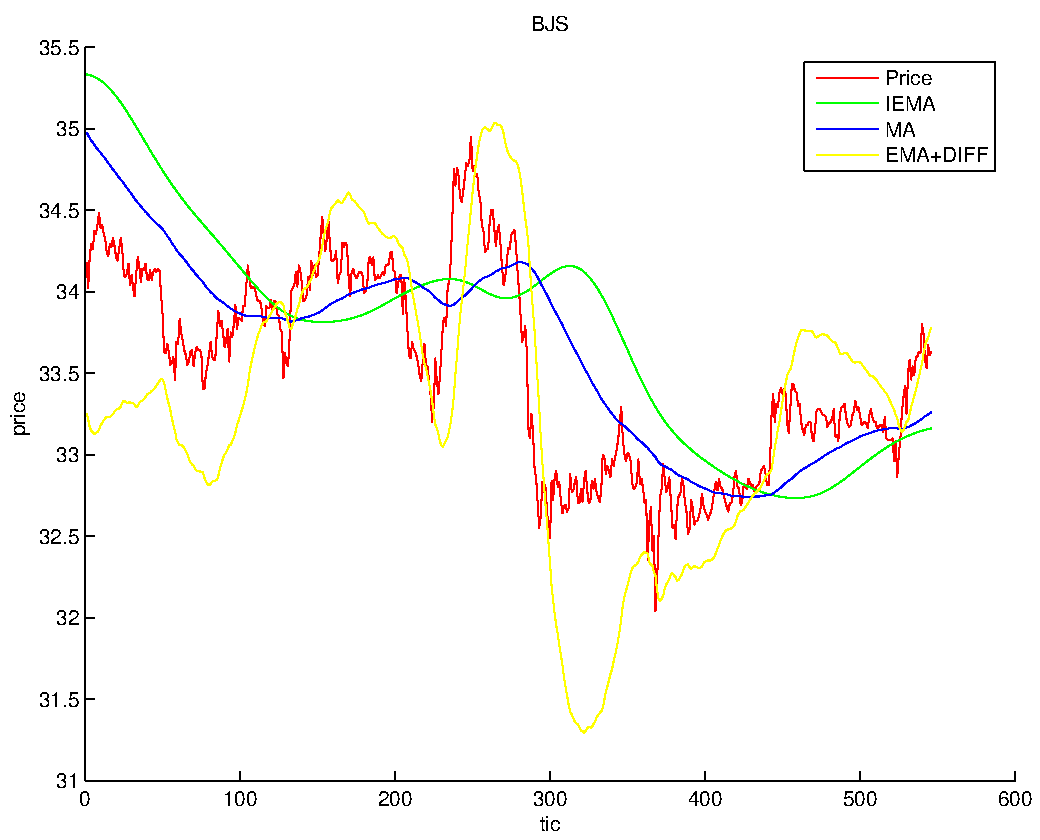
\includegraphics[width=4.0cm,height=4.0cm]{images/RealTimeFinancialTSMining/klTimeSeries/BJSFilteredPriceSeries.pdf}  \\
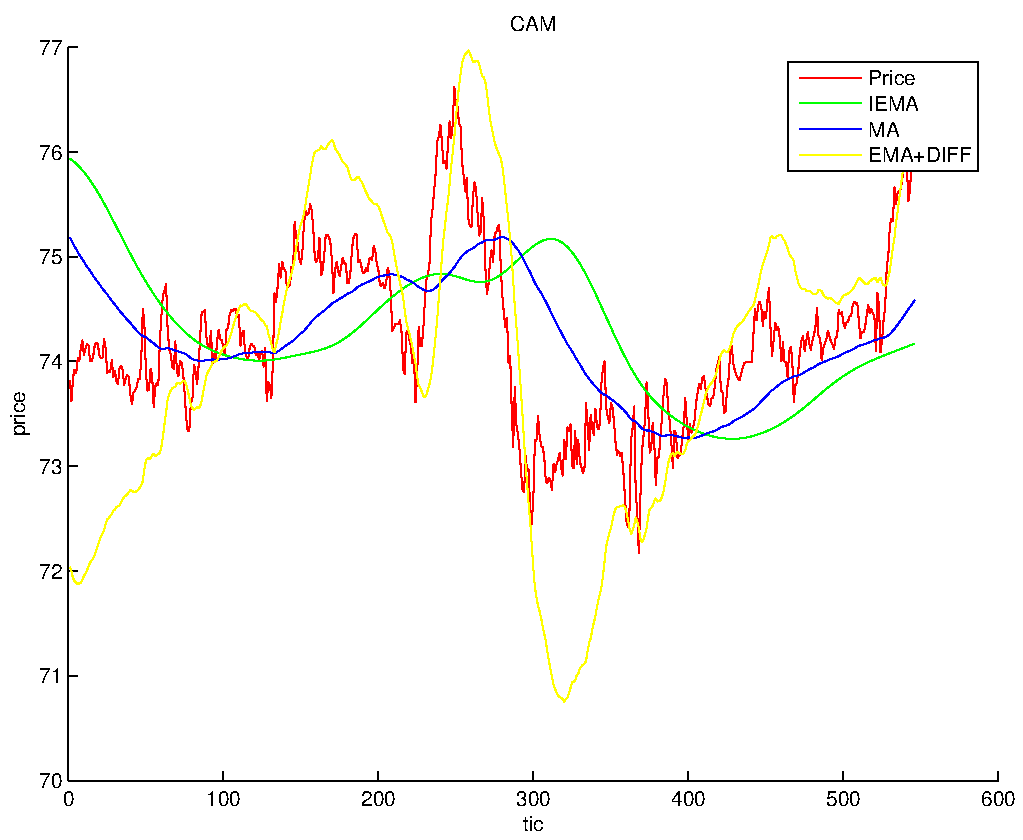
\includegraphics[width=4.0cm,height=4.0cm]{images/RealTimeFinancialTSMining/klTimeSeries/CAMFilteredPriceSeries.pdf}   &
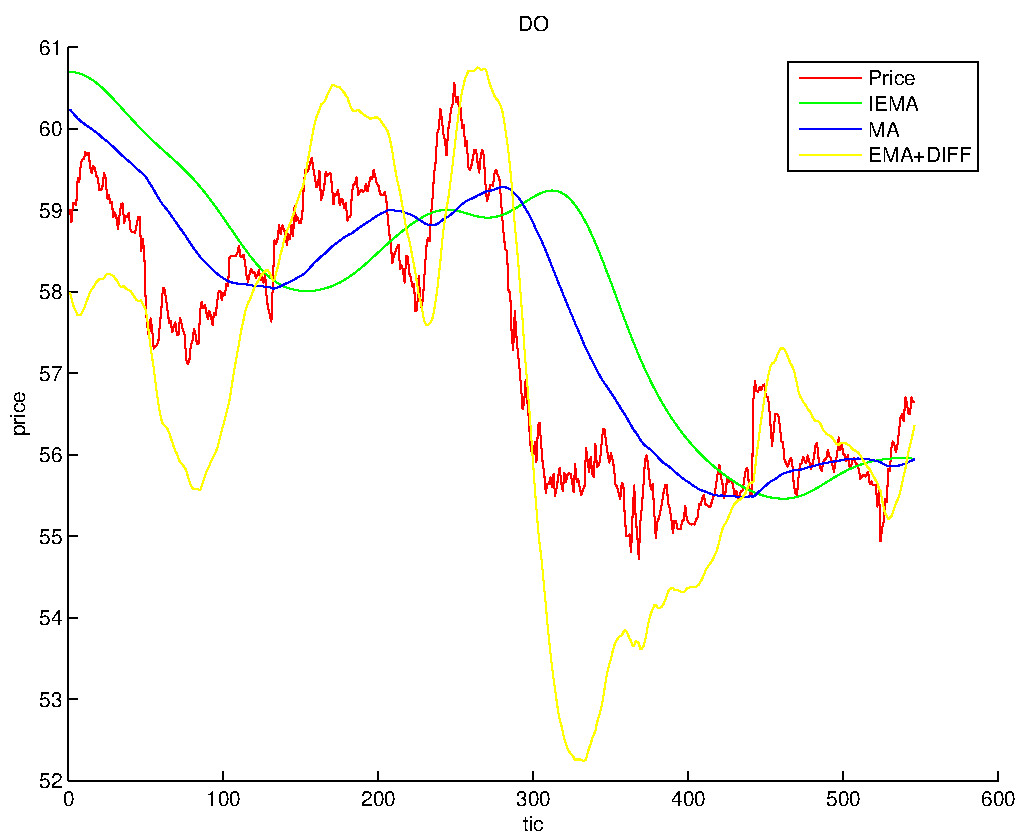
\includegraphics[width=4.0cm,height=4.0cm]{images/RealTimeFinancialTSMining/klTimeSeries/DOFilteredPriceSeries.pdf}  &
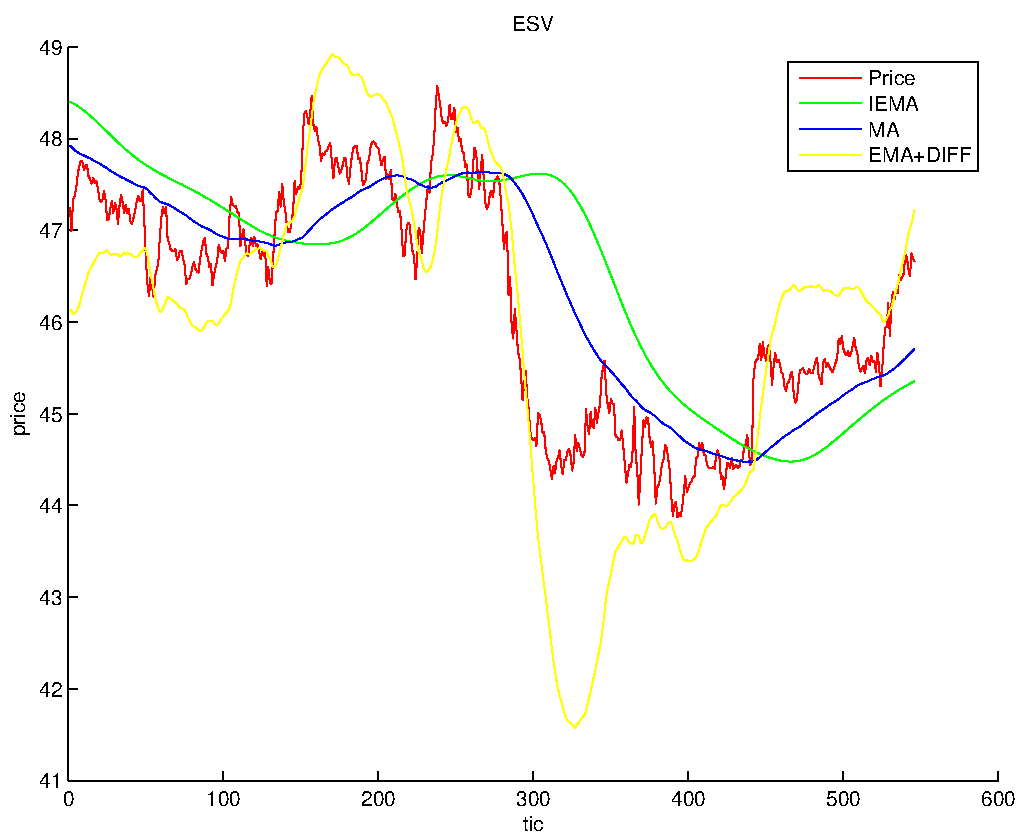
\includegraphics[width=4.0cm,height=4.0cm]{images/RealTimeFinancialTSMining/klTimeSeries/ESVFilteredPriceSeries.pdf}  &
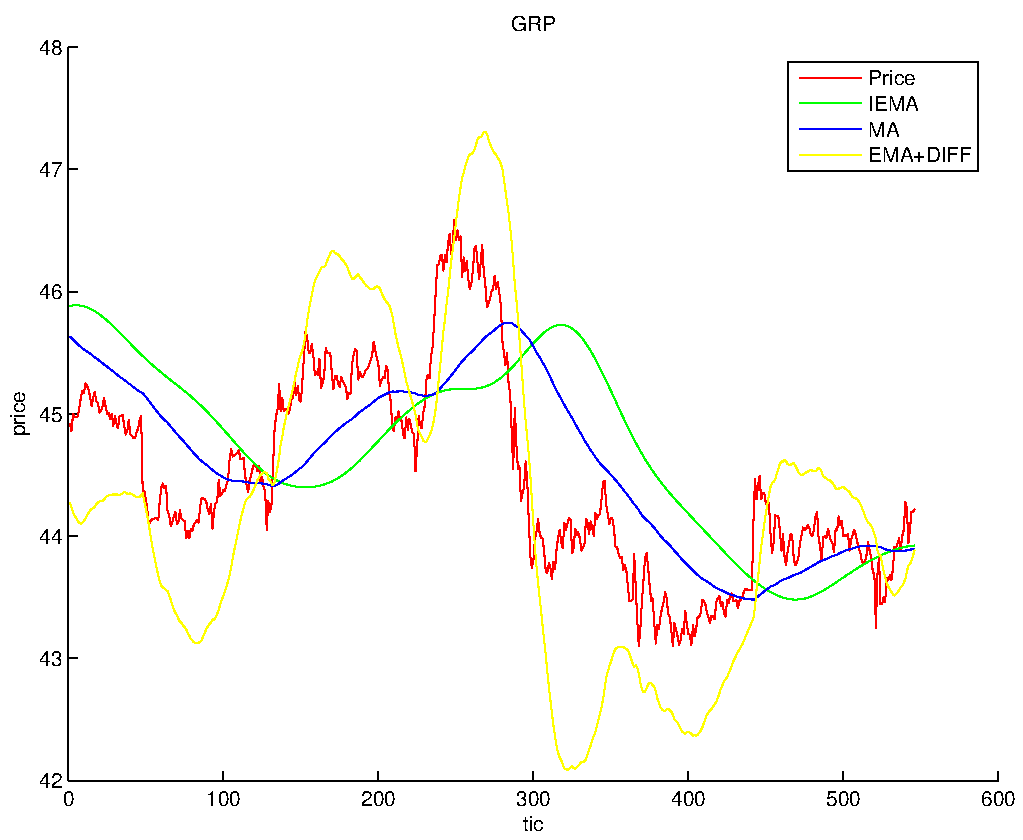
\includegraphics[width=4.0cm,height=4.0cm]{images/RealTimeFinancialTSMining/klTimeSeries/GRPFilteredPriceSeries.pdf}   \\
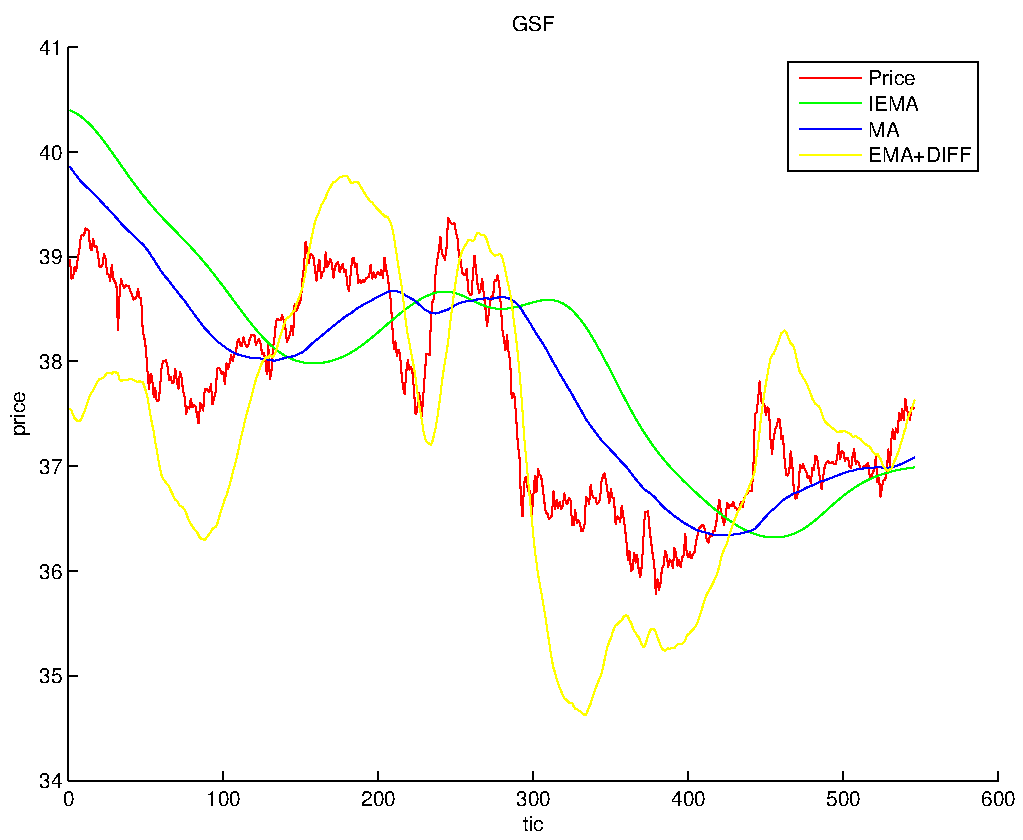
\includegraphics[width=4.0cm,height=4.0cm]{images/RealTimeFinancialTSMining/klTimeSeries/GSFFilteredPriceSeries.pdf}  &
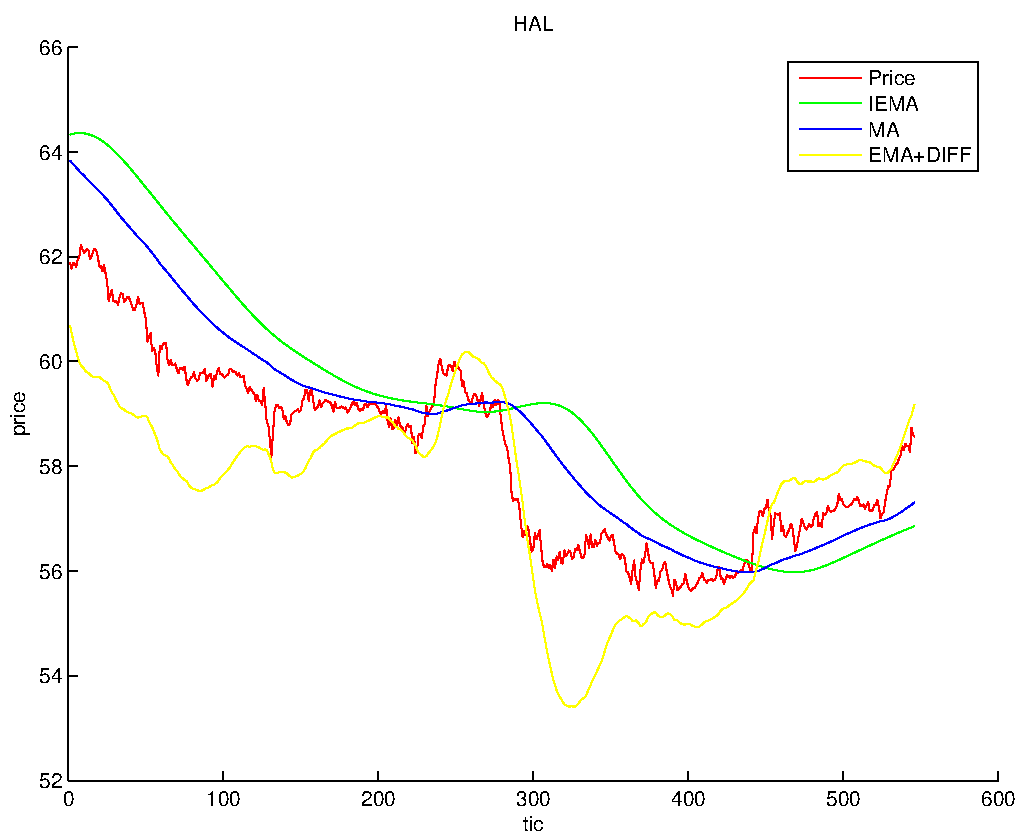
\includegraphics[width=4.0cm,height=4.0cm]{images/RealTimeFinancialTSMining/klTimeSeries/HALFilteredPriceSeries.pdf}  &
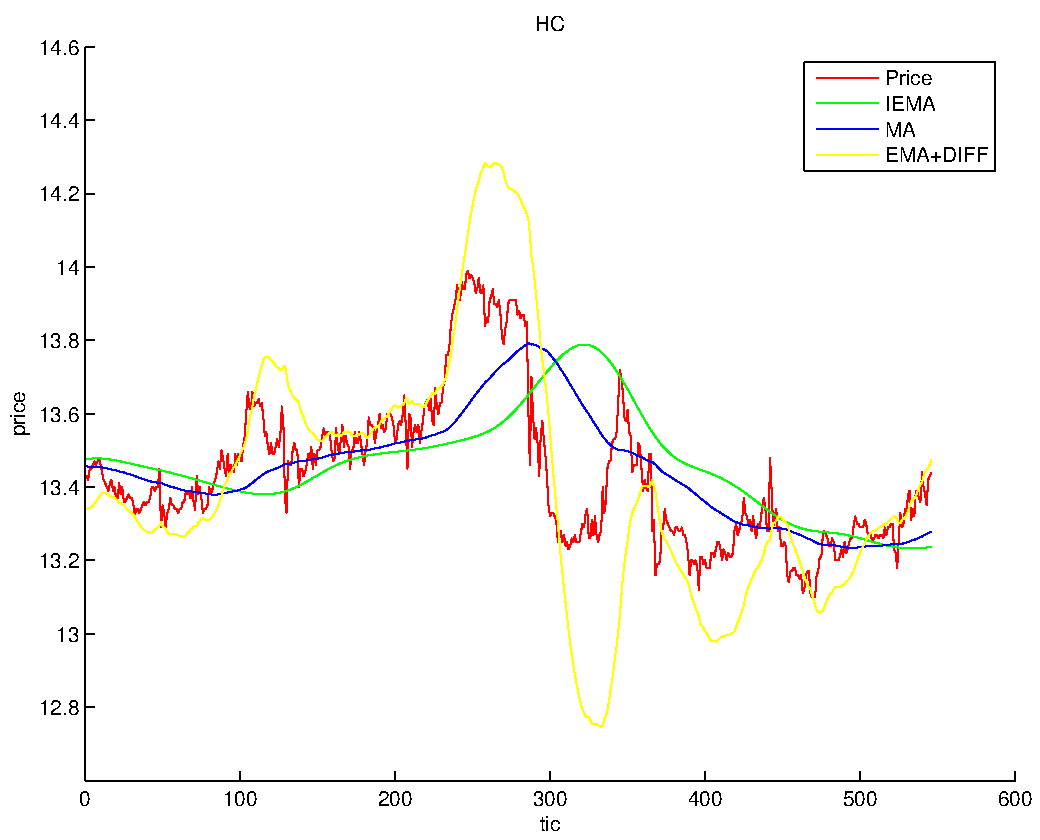
\includegraphics[width=4.0cm,height=4.0cm]{images/RealTimeFinancialTSMining/klTimeSeries/HCFilteredPriceSeries.pdf}   &
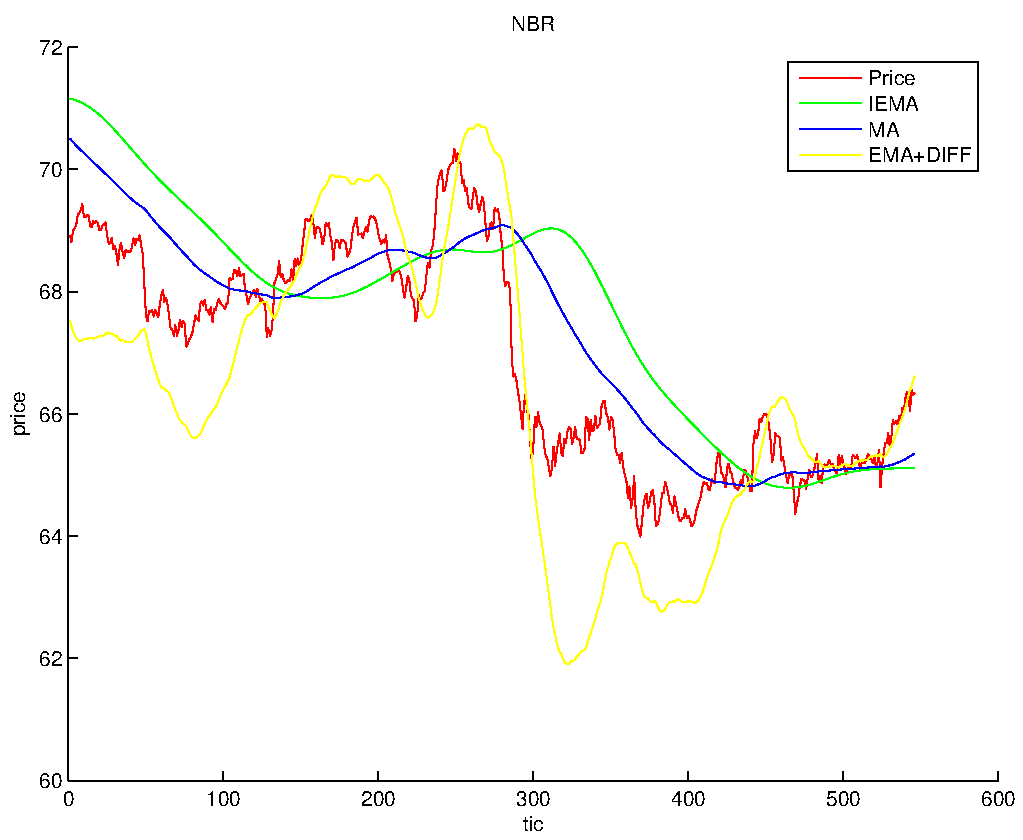
\includegraphics[width=4.0cm,height=4.0cm]{images/RealTimeFinancialTSMining/klTimeSeries/NBRFilteredPriceSeries.pdf}  \\
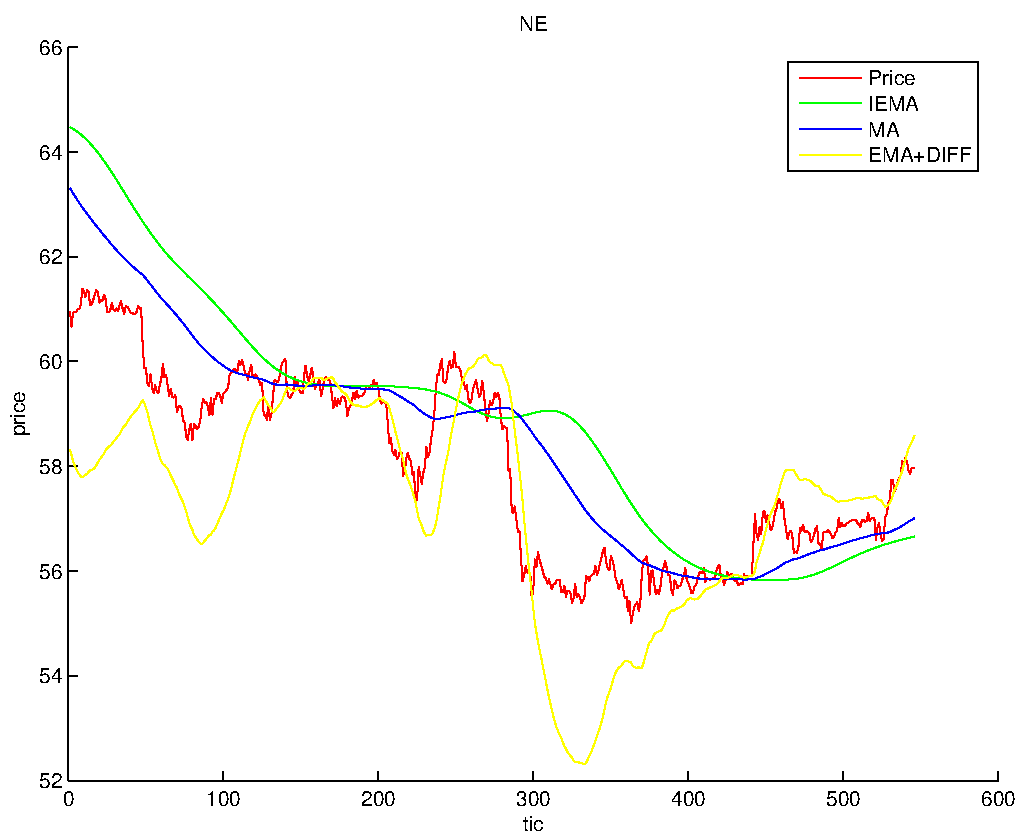
\includegraphics[width=4.0cm,height=4.0cm]{images/RealTimeFinancialTSMining/klTimeSeries/NEFilteredPriceSeries.pdf}    &
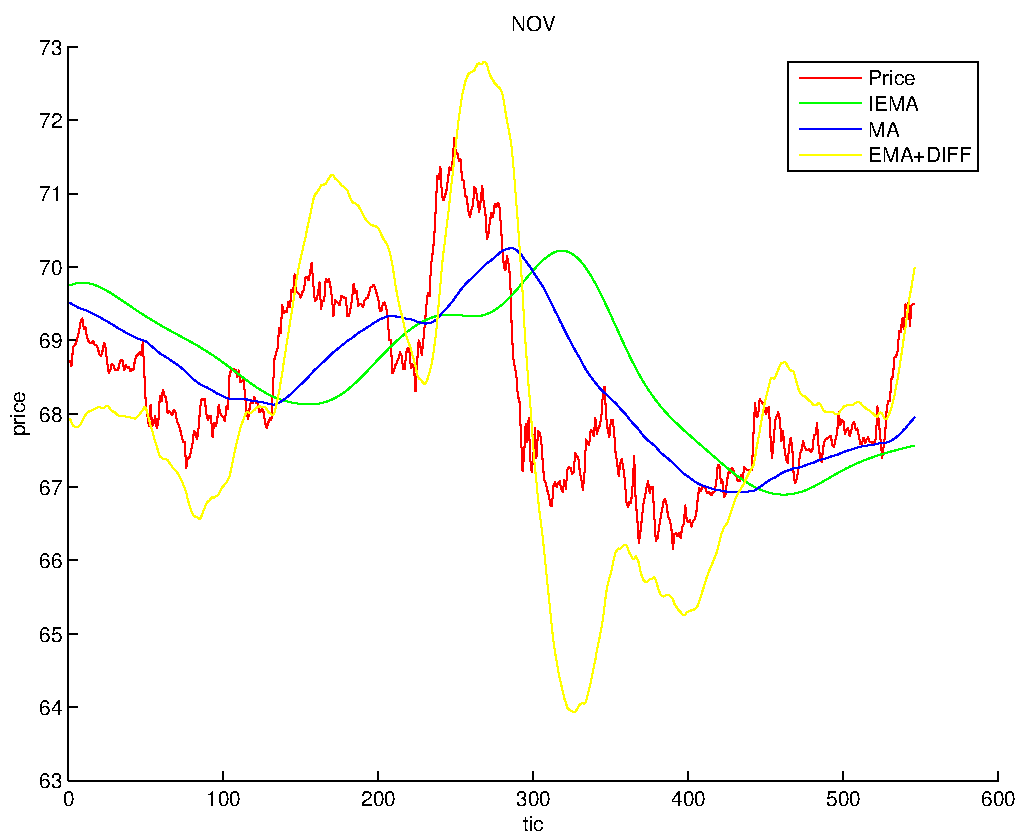
\includegraphics[width=4.0cm,height=4.0cm]{images/RealTimeFinancialTSMining/klTimeSeries/NOVFilteredPriceSeries.pdf}   &
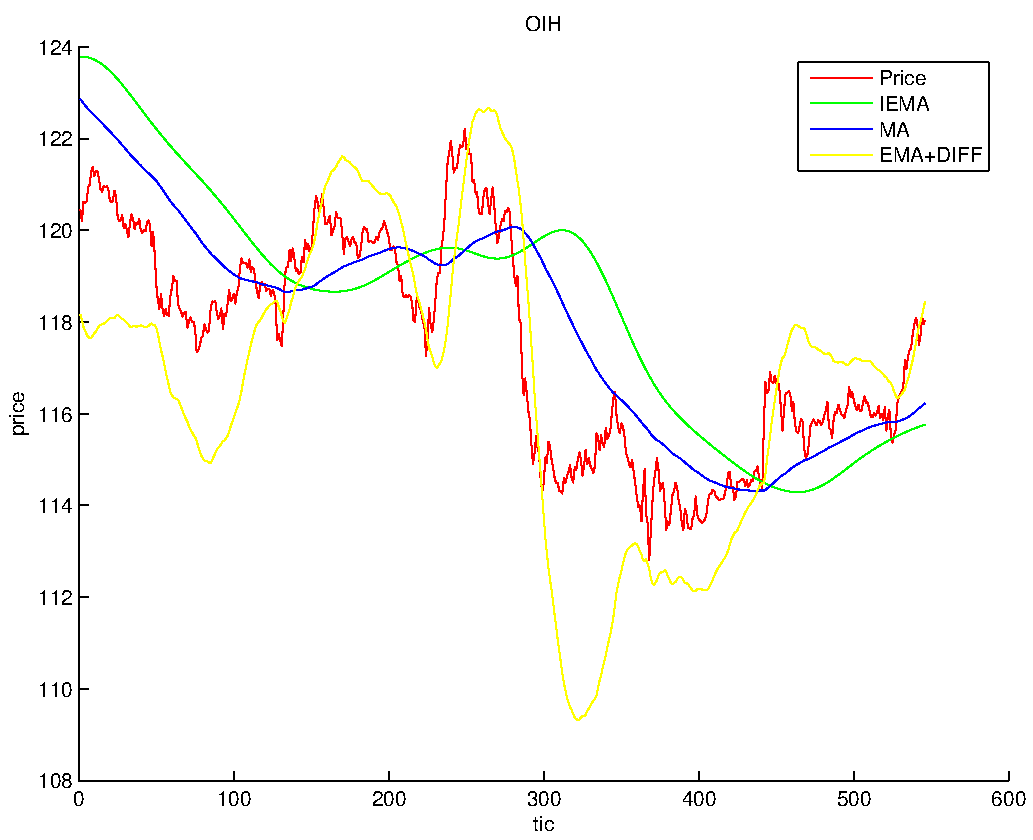
\includegraphics[width=4.0cm,height=4.0cm]{images/RealTimeFinancialTSMining/klTimeSeries/OIHFilteredPriceSeries.pdf}   &
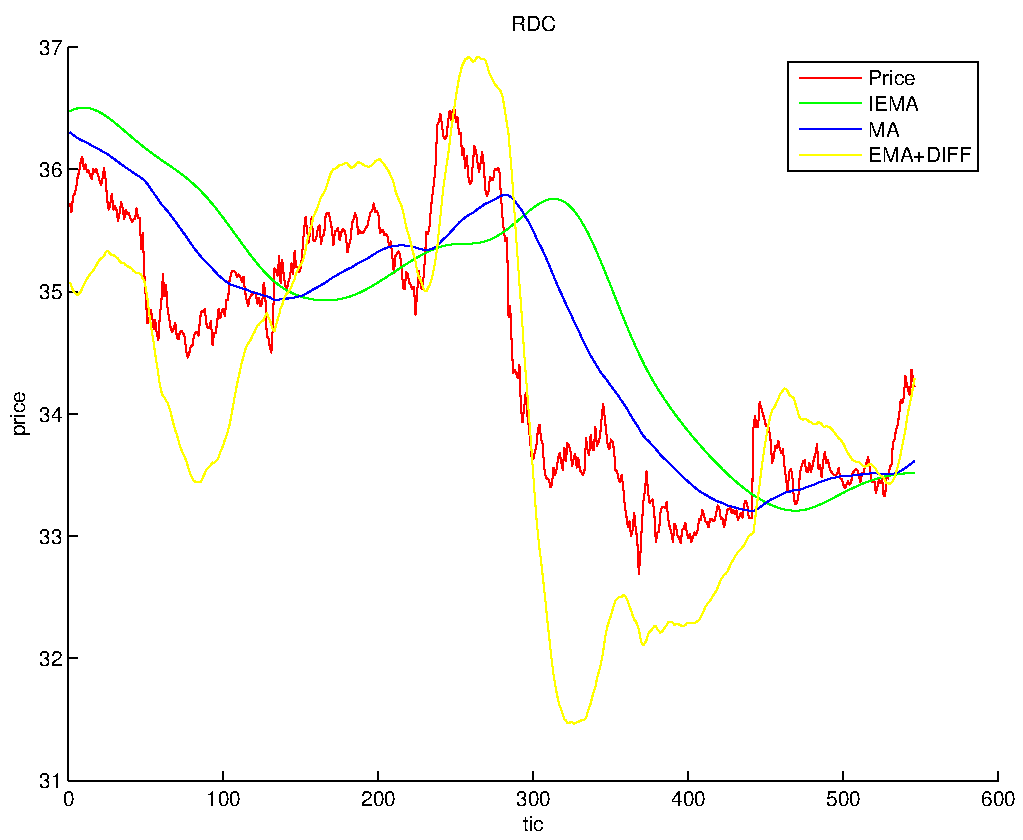
\includegraphics[width=4.0cm,height=4.0cm]{images/RealTimeFinancialTSMining/klTimeSeries/RDCFilteredPriceSeries.pdf}   \\
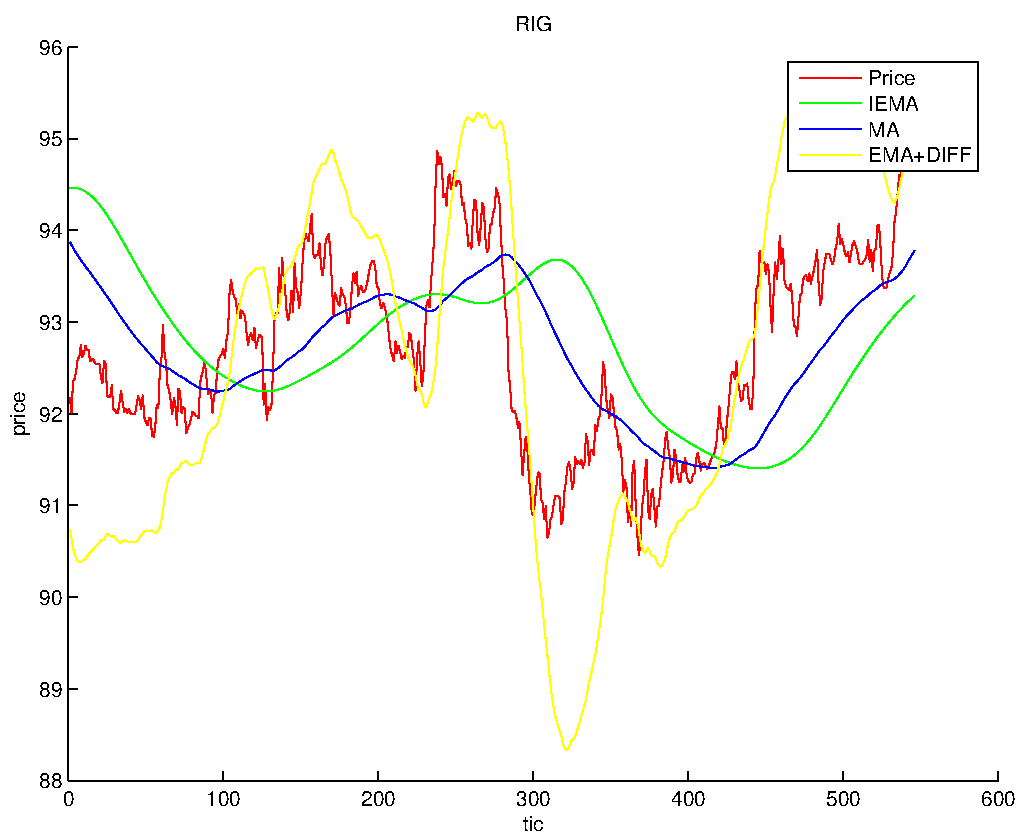
\includegraphics[width=4.0cm,height=4.0cm]{images/RealTimeFinancialTSMining/klTimeSeries/RIGFilteredPriceSeries.pdf}   &
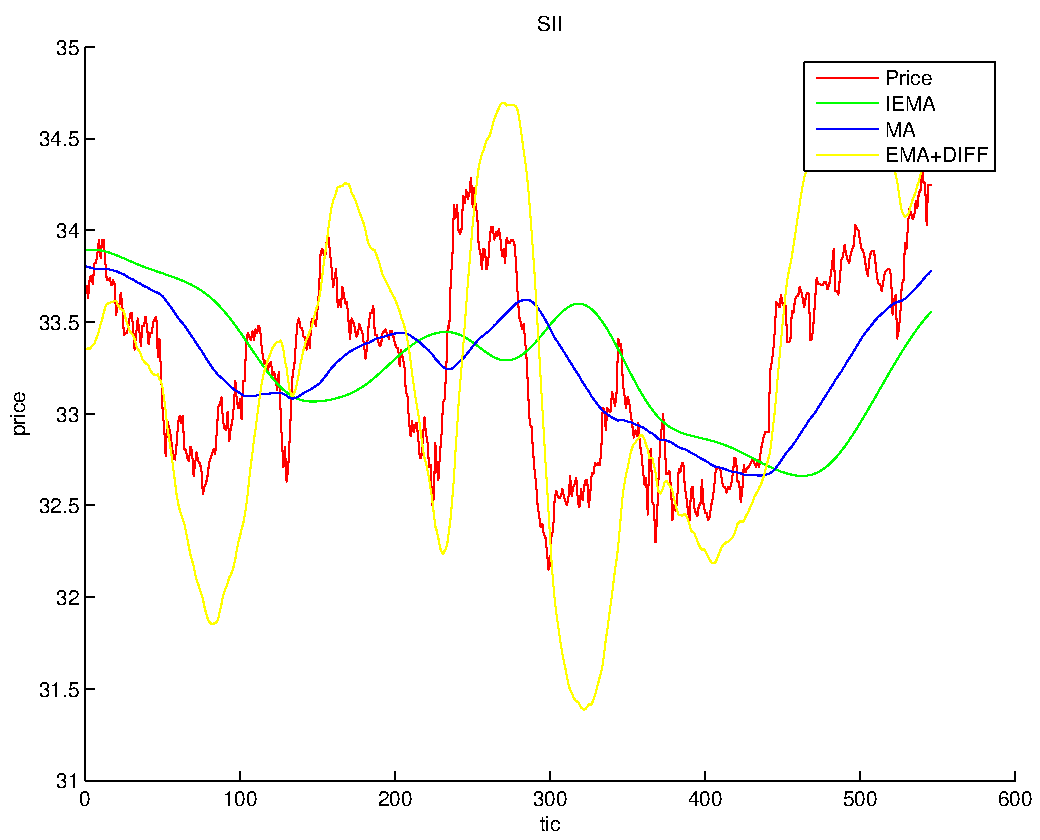
\includegraphics[width=4.0cm,height=4.0cm]{images/RealTimeFinancialTSMining/klTimeSeries/SIIFilteredPriceSeries.pdf}   &
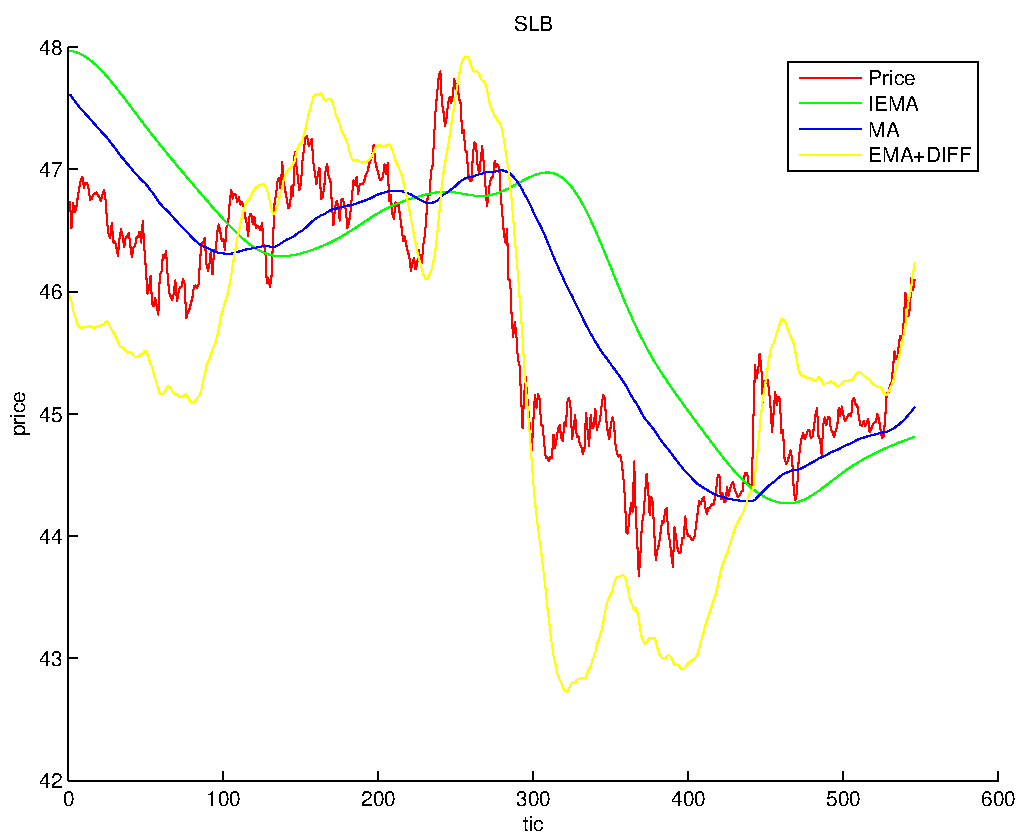
\includegraphics[width=4.0cm,height=4.0cm]{images/RealTimeFinancialTSMining/klTimeSeries/SLBFilteredPriceSeries.pdf}   &
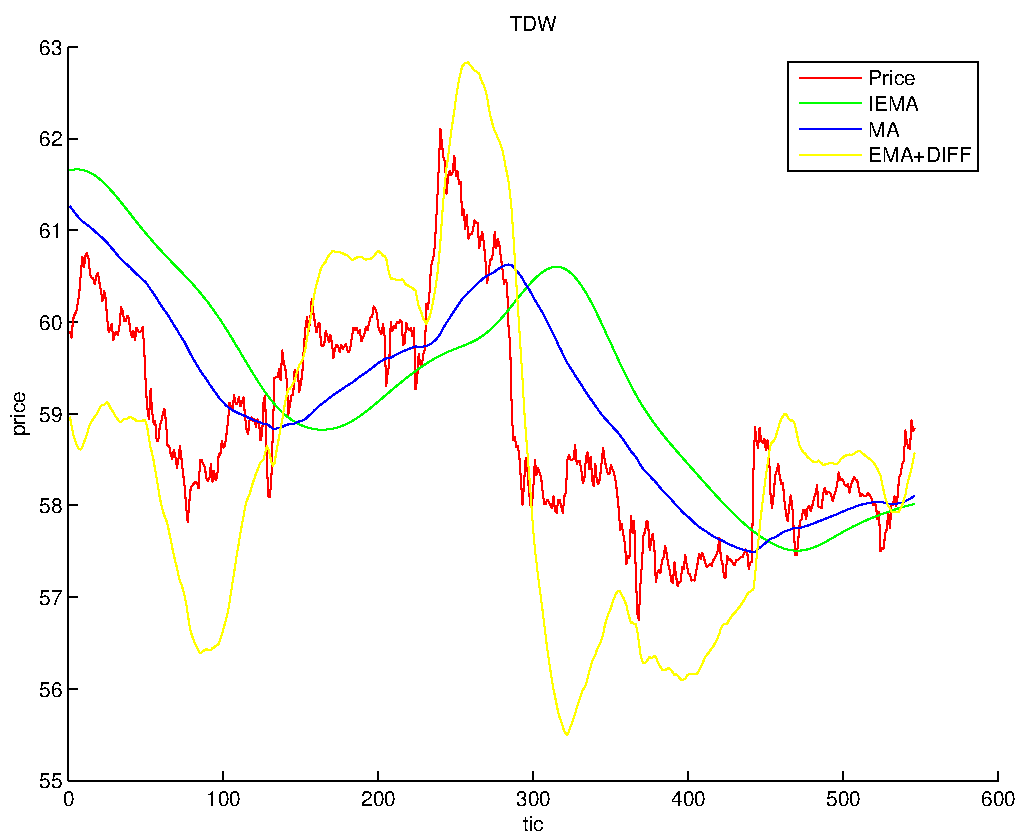
\includegraphics[width=4.0cm,height=4.0cm]{images/RealTimeFinancialTSMining/klTimeSeries/TDWFilteredPriceSeries.pdf}
\end{tabular}
